\section{Movimento OpenData}
% Filosofia
%Con il termine Open Data (o dati aperti) si definisce sia la filosofia che la pratica, che prevedono l'esistenza di diverse tipologie di dati accessibili liberamente a tutti, senza restrizioni derivanti da brevetti o copyright, fatta eccezione per le licenze che obbligano a citarne la fonte o al rilascio dei dati modificati con lo stesso tipo di licenza.

Partecipazione, Democrazia, Comunit�, Diritti� sono solo alcune delle parole che vengono associate agli OpenData. Ci� pu� avvenire attraverso il ricorso alle nuove tecnologie dell'informazione e della comunicazione, sulla base delle esperienze positive gi� sperimentate in altri movimenti e comunit� �open�, quali l'\textit{open source}, l'\textit{open access} e l'\textit{open content}. Negli anni la pratica e l'ideologia che caratterizza i dati aperti si � ben consolidata, ma solo recentemente � nata una nuova accezione legata maggiormente al mondo di Internet, che diventa il canale principale di diffusione dei dati stessi, e con essa si identifica il termine �Open Data�. Secondo wikipedia \cite{wiki-datiaperti} per open data si intendono \textit{�alcune tipologie di dati liberamente accessibili a tutti, privi di brevetti o altre forme di controllo che ne limitino la riproduzione e le cui restrizioni di copyright eventualmente si limitano ad obbligare di citare la fonte o al rilascio delle modifiche allo stesso modo.}\\

\begin{figure}[htbp]
   \centering
   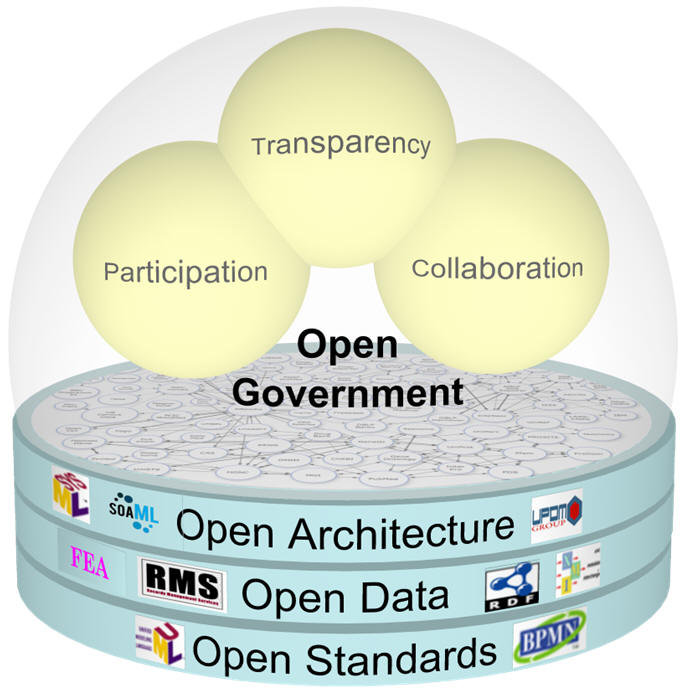
\includegraphics[scale=0.80]{img/OpenGovernment.jpg}
   \caption{Pilastri dell�OpenGovernment}
   \label{fig:OpenGovernment}
\end{figure}

In fiugra \ref{fig:OpenGovernment} si vede come Open Data sia uno dei pilastri dell'Open Government, ovvero l'idea in base alla quale la pubblica amministrazione deve essere aperta ai cittadini in termini di trasparenza, di collaborazione e di partecipazione diretta al processo decisionale. \'E bene dunque evidenziare che Open Data di per se non vuol dire \textit{e-participation} (partecipazione in processi di governo e di governance) o \textit{e-democracy}, ma insieme con loro costituiscono i pilastri dell'Open Government.

Ci� comporta che i dati siano messi a disposizione dalla Pubblica Amministrazione in sola lettura da parte degli utenti, i quali li utilizzano in base alle loro esigenze:
\begin{itemize}
\item \textbf{Cittadini}: per misurare le performance e la trasparenza della Pubblica Amministrazione (es. dati di bilancio), o per informazione (es. orari mezzi pubblici, sportelli sanitari, ...).
\item \textbf{Civil Hackers}: per spirito civico sviluppano app basate sui open data per intenti civici, trovando il meccanismo per mettere facilmente a disposizione dei cittadini i dati pubblici.
\item \textbf{Giornalisiti}: per cercare informazioni legati a interessi particolari (es. lugli della citt� statisticamente con maggior criminalit�).
\item \textbf{Imprese}: principalmente per analisi di mercato (es. esercizi sul territorio interessati a un prodotto) o per produzione di software che sfrutta l�informazione presente nei dati.
\item \textbf{Pubblica amministrazione}: per migliorare le scelte decisionali (es. un tasso di malattia anomalo pu� essere correlato alla presenza di sostanze tossiche).
\end{itemize}

\newpage
I dati del governo sono considerati aperti se sono resi pubblici in modo da rispettare gli \textbf{8 principi dell�Open Governament Data} definiti da un gruppo di 30 persone nel 2007 a Sebastopol, California \cite{open-governament-data} :
\begin{enumerate}
\item \textbf{Completi}: Tutti i dati pubblici sono resi disponibili. Sono dati che non sono soggetti a limitazioni di privacy, di sicurezza o limitazioni di privilegio.
\item \textbf{Primari}: I dati vengono raccolti alla fonte, con il pi� alto possibile livello di �gnaularit��, non in forme aggregate o modificate.
\item \textbf{Tempestivi}: Dati sono resi disponibili in tempi necessari a preservarne il valore e devono essere mantenuti aggiornati.
\item \textbf{Accessibili}: I dati sono disponibili al maggior numero di utenti per i pi� vari scopi.
\item \textbf{Processabili}: I dati vengono adeguatamente strutturati per consentire l'elaborazione automatizzata.
\item \textbf{Non discriminatori}: I dati sono disponibili a chiunque, senza necessit� di registrazione.
\item \textbf{Non proprietari}: I dati sono disponibili in un formato su cui nessun ente ha l�esclusivo controllo.
\item \textbf{Liberi da licenza}:  I dati non sono soggetti a diritti d'autore, brevetti, marchi o segreto commerciale. Possono essere ammesse ragionevoli restrizioni di privacy, sicurezza e privilegio.
\end{enumerate}
In aggiunta agli 8 principi � inoltre importante rendere i dati:
\begin{itemize}
\item \textbf{Riutilizzabili}: Gli utenti devono essere messi in condizione di riutilizzare e integrare i dati, in modo da creare nuove risorse, applicazioni, programmi e servizi di pubblica utilit�.
\item \textbf{Ricercabili}: Facilmente identificabili in rete e facilmente indicizzabili dai motori di ricerca.
\item \textbf{Permanenti}: Le caratteristiche sopra descritte devono caratterizzare i dati nel corso della loro intera vita sul Web.
\end{itemize}

I dati che son stati resi disponibili sono quindi di diverso formato e posso riguardare statistiche o censimenti, dati sensibili accorpati, dati georeferenziati o materiale multimediale.

% scala 5 stelle
\subsection{Scala 5 stelle}
Tim Berners Lee in un suo testo del 2006, successivamente integrato nel 2010 \cite{BernersLee-LinkedData}, per incoraggiare i governi ed altri enti pubblici a rilasciare i dati in formato aperto, introdusse il concetto di \textbf{Dati a 5 stelle}. I concetti trattati nel articolo sono il \textit{Semantic Web} e i \textit{Linked Open Data}, ovvero un particolare tipo di dato strutturato semanticamente che viene pubblicato in rete con licenze di consultazione e d�uso poco restrittive (quali le licenze Creative Commons o le licenze nazionali) e che viene classificato secondo la scala a 5 stelle.\\

\begin{figure}[htbp]
   \centering
   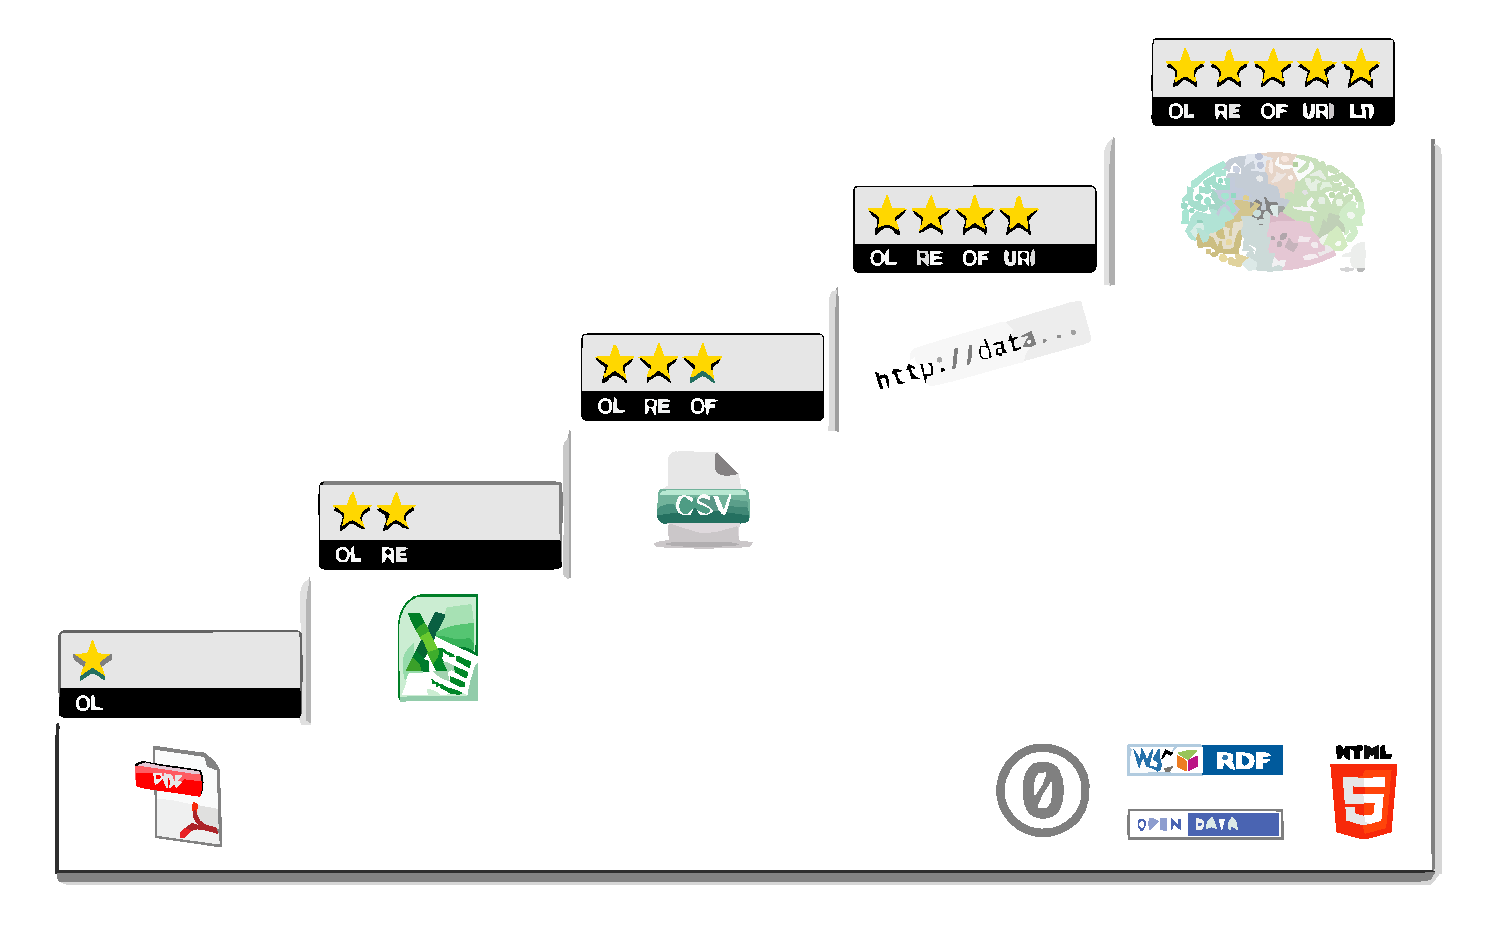
\includegraphics[scale=1.80]{img/5star-steps}
   \caption{Scala a 5 stelle}
   \label{fig:5star-steps}
\end{figure}

La scala a 5 stelle (fig. \ref{fig:5star-steps}) vuole misurare quanto i dati siano aperti e accessibili, assegnando le stelle secondo i seguenti criteri:

%\begin{table}[htbp]
\begin{center}
\begin{tabularx}{\textwidth}{r X}
no star & \textbf{Web data} (in qualsiasi formato) senza nessuna licenza open\\
\ding{72} & Il dato � disponibile sul Web (in qualsiasi formato) con una \textbf{licenza aperta}\\
\ding{72} \ding{72} & Il dato � disponibile in un \textbf{rformato strutturato} (ad esempio un Excel invece della scansione di una tabella) in modo che possa essere iutilizzato\\
\ding{72} \ding{72} \ding{72} & Il dato � in un \textbf{formato non proprietario} (ad esempio un CSV invece di un Excel)\\
\ding{72} \ding{72} \ding{72} \ding{72} & Il dato utilizza gli \textbf{URI} per identificare gli oggetti, in modo che le persone possano far riferimento alle sue risorse e fare uso di RDF\\
\ding{72} \ding{72} \ding{72} \ding{72} \ding{72} & Il \textbf{dato} � \textbf{collegato} ad altri dati per fornire un contesto\\
\end{tabularx}
\end{center}
%\end{table} 

% Obama, ...
\subsection{Open Data in ambito governativo}
Una grossa spinta all'affermazione del movimento Open Data in ambito governativo � stata data dal presidente degli Stati Uniti d'America \textbf{Barack Obama} con la promulgazione di una Direttiva sull'Open government nel dicembre 2009 \cite{Direttiva-OpenGovernament}:

\begin{quoting}
Fin dove possibile e sottostando alle sole restrizioni valide, le agenzie devono pubblicare le informazioni on line utilizzando un formato aperto (open) che possa cio� essere recuperato, soggetto ad azioni di download, indicizzato e ricercato attraverso le applicazioni di ricerca web pi� comunemente utilizzate. Per formato open si intende un formato indipendente rispetto alla piattaforma, leggibile dall�elaboratore e reso disponibile al pubblico senza che sia impedito il riuso dell�informazione veicolata.
\end{quoting}

Alla direttiva � stato dato seguito con la pubblicazione sul sito web \url{Data.gov} di molti dati in formato aperto. Il portale ha infatti lo scopo di raccogliere tutte le informazioni rese disponibili dagli enti statunitensi. \cite{wiki-datiaperti}
Nel maggio 2013 Barack Obama ha firmato un nuovo ordine esecutivo \cite{WhiteHouse-OpenData} che obbliga tutte le agenzie governative ad adottare dati in formato aperto compatibili anche con le future infrastrutture informatiche che verranno adottate negli USA. Le pubbliche amministrazioni dovranno assicurarsi, dove � legalmente consentito, che i dati vengano rilasciati in modo tale da risultare facilmente accessibili e utilizzabili.\\

% Italia
\subsection{Open Data in Italia}
\textbf{In Italia} la spinta iniziale � stata data tra il 2007 e il 2010 dalla volont� di alcune amministrazioni locali che han voluto partecipare al progetto \href{http://www.openstreetmap.org/}{OpenStreetMap}, il quale crea e fornisce dati cartografici, come ad esempio mappe stradali, libere e gratuite a chiunque ne abbia bisogno.
I comuni coinvolti, insieme a dei volontari, hanno condiviso i dati dei propri stradari sotto licenza aperta.

Nel giugno 2010 Renato Brunetta, l'allora Ministro per la pubblica amministrazione e l'innovazione, dichiar� in un intervista l'intenzione di realizzare un portale italiano dell�Open data seguendo il modello dei datagov anglosassoni entro la fine dell'anno. Il 18 Ottobre 2011 il portale \url{dati.gov.it} � stato messo on line.

Nel maggio 2010 la regione Piemonte ha realizzato il proprio portale regionale \url{dati.piemonte.it}. Il sito � ancor oggi una delle esperienze nazionali con la miglior riuscita.
Nel 2011 la regione Emilia-Romagna ha seguito l'esempio piemontese.

A partire da settembre 2011 il Comune di Firenze, grazie anche alla spinta del suo Sindaco Matteo Renzi, ha realizzato il proprio portale \url{opendata.comune.fi.it} rilasciando un dataset al giorno nella fase iniziale. Inoltre Firenze � stato il primo comune a testare OpenBilancio, una visualizzazione dei dati che vuole essere comprensibile da tutti.

Nel marzo 2012 � stata rilasciata la seconda versione della licenza progettata per i dati delle Pubbliche Amministrazioni: Italian Open Data License, indicata come IODL v2.0 \cite{IODL2.0}, priva del vincolo "condividi-allo-stesso-modo" e con la sola richiesta di attribuzione della fonte per il riutilizzo dei dati. \cite{wiki-datiaperti}